\documentclass{article}
\usepackage{graphicx}
\usepackage{cgw06}
\usepackage{epsf}
\usepackage{polski}
\usepackage[T1]{fontenc}
\usepackage[utf8]{inputenc}
\usepackage{hyperref}
\usepackage{xcolor}
\usepackage[all]{hypcap}
\usepackage{color}
\usepackage{mdframed}
\usepackage{titletoc}
\usepackage{listings}
\usepackage{mathtools}

\definecolor{dark-red}{rgb}{0.5,0,0}
\definecolor{dark-green}{rgb}{0,0.5,0}
\definecolor{dark-blue}{rgb}{0,0,0.5}
\hypersetup{
    colorlinks,
    linkcolor={dark-blue},
    urlcolor={dark-blue},
    citecolor={dark-green}
}

\lstdefinestyle{customc}{
  belowcaptionskip=1\baselineskip,
  breaklines=true,
  frame=L,
  xleftmargin=\parindent,
  language=Pascal,
  showstringspaces=false,
  basicstyle=\footnotesize\ttfamily,
  keywordstyle=\bfseries\color{green!40!black},
  commentstyle=\itshape\color{purple!40!black},
  identifierstyle=\color{blue},
  stringstyle=\color{orange},
}

\lstset{escapechar=@,style=customc}

\begin{figure}[ht!]
\centering

\includegraphics[width=90mm]{AGH.jpg}
\label{overflow}
\end{figure}
\title {Skrzyżowania ++}

\author{Projekt realizowany w ramach laboratorium z Badań Operacyjnych \\* \\* Piotr Skibiak, Tomasz Kwiecień, Marcin Nowak, Ksawery Głaz, Paweł Łabno}
\institute{AGH, Wydział IEiT, Informatyka, rok 2014}
\begin{document}

\maketitle

\begin{abstract}
Projekt ma na celu skrócenie oczekiwania samochodów na skrzyżowaniach, poprzez zastosowanie optymalnego ustawienia czasu świateł. Optymalne (albo prawie optymalne) ustawienie świateł wyznaczane jest poprzez użycie jednego z algorytmów stadnych - algorytmu kukułki.   
\end{abstract}

\newpage
\renewcommand*\contentsname{Spis Treści}
\tableofcontents
\setcounter{tocdepth}{3}

\newpage

\section{Przedstawienie problemu}
    Od początku XX wieku rośnie ilość samochodów na ulicach. Według zamierzeń Henrego Forda każdy Amerykanin powinien posiadać swój samochód. Jego wizja została już w dużej części zrealizowana, jednakże przyniosło to ze sobą pewne negatywne skutki. W miastach (zwłaszcza tych wielkich) często spotyka się zjawisko jakim są zakorkowane ulice pełne samochodów. Jednak każda ulica ma inne natężenie ilości samochodów w różnych porach dnia, a światła na skrzyżowaniach mają stałe czasy świecenia. W czasie tak zwanych godzin szczytu przez jedne ulice przejeżdża więcej samochodów niż przez inne, co powoduje korki na drogach. Spotykanym zjawiskiem jest sytuacja kiedy droga o mniejszym natężeniu jest uprzywilejowana. Można by jednak upłynnić ten ruch poprzez wydłużenie czasu świecenia świateł zielonych dla bardziej uczęszczanych ulic, a skrócenie go dla tych mniej uczęszczanych. I właśnie tym zajmuje się nasz program. Czyli badaniem w danych godzinach natężenia ruchu na danych ulicach i optymalizowanie czasów świecenia świateł tak aby ten ruch był płynniejszy dla całego wybranego (narysowanego) obszaru. W tym celu korzystamy z algorytmu kukułki, który wyznacza optymalne czasy świecenia świateł dla poszczególnych skrzyżowań.

\section{Cele projektu}
    Projekt ma na celu umożliwienie użytkownikowi znalezienie optymalnego ustawienia czasów świecenia świateł (światła zielonego i czerwonego) w sieci skrzyżowań ustalonych przez użytkownika. Aplikacja powinna dać użytkownikowi możliwość ręcznego wprowadzenia sieci skrzyżowań, zapisu konfiguracji do pliku, lub wczytania wcześniej zapisanej. 

\section{Wstępne założenia}

\subsection{Środowisko Implementacji}
    Aby pogodzić potrzebę szybkiego wykonywania symulacji, oraz zdążyć wykonać projekt w przeznaczonym do tego czasie, językiem wybranym do implementacji jest Java w siódmej wersji. Ustaliliśmy, że aby zmniejszyć prawdopodobieństwo wystąpienia niespójności związanej z wykorzystywaniem różnych narzędzi, aplikacja będzie pisana przy pomocy Eclipse IDE. 

\subsection{Praca w zespole}
    Praca grupowa była wspomagana poprzez wykorzystanie sytemu kontroli wersji GIT \url{<https://github.com/blostic/BO>}, oraz poprzez utworzenie Google Doc'a projektu. W trakcie realizacji przeprowadziliśmy również kilka spotkań mających na celu, kontrolę przebiegu prac, wyjaśnienie wątpliwości / niejasności wykrytych w trakcie iteracji, a także przydział kolejnych zadań.


\subsection{Założenia projektowe}
    W naszym projekcie zastosowany został szereg uproszczeń. Staraliśmy się, aby przyjęte założenia nie ingerowały znacząco w strukturę problemu i żeby otrzymane rezultaty z powodzeniem mogły zostać zastosowane do realnych problemów. Pominęliśmy przede wszystkim czas świecenia żółtego światła przy zmianie z czerwonego na zielone oraz odwrotnie. Nie są rozpatrywane przypadki, gdy samochód na skrzyżowaniu zawraca lub możliwy jest ruch bezkolizyjny kilku samochodów. Pomnieliśmy także przejścia dla pieszych oraz obecność innych uczestników ruchu niż pojazdy kołowe. Uproszczenie, które również zostało przyjęte w aplikacji, jest istnienie tylko i wyłącznie skrzyżowań 4 wlotowych. Skrzyżowania posiadające mniejszą liczbę dróg wejściowych można jednak z powodzeniem symulować przy pomocy dróg o natężeniu 0. Każde połączenie jest traktowane jako droga dwukierunkowa jednopasmowa.

\section{Opis logiki}
  Logika biznesowa aplikacji składa się z kilku klas, które umożliwiają tworzenie obiektów takich jak: Generatory, Skrzyżowania, Drogi i Samochody. Z tych obiektów składa się model, na którym będzie przeprowadzana symulacja. 

\subsection{Klasa Generator}
    Obiekt, który jest instancją tej klasy jest zakończeniem drogi, których jeden z końców nie jest podłączony do żadnego ze skrzyżowań. Zadaniem tego obiektu jest tworzenie nowych samochodów pojawiających się na mapie oraz usuwanie tych wyjeżdżających z mapy. Klasa posiada metodę moveVehicles odpowiedzialną za pojawianie się i znikanie samochodów na mapie. Klasa posiada  niedeterministyczną metodę, która decyduje, czy obiekt Generator powinien w danym momencie stworzyć obiekt Vehicle.

\subsection{Klasa Junction}
    Jest to klasa abstrakcyjna dla Klas Intersection i Generator. Posiada pola przechowujące współrzędne tych obiektów na mapie, oraz Listy dróg wejściowych i wyjściowych. Posiada metodę, która dodaje na każdą ulicę wychodzącą z tego skrzyżowania stałą liczbę samochodów. Liczba ta jest zależna od ustalonego wcześniej natężenia ruchu na danej drodze.
\subsection{Klasa Intersection}
    Instancja te klasy odpowiada za obsługę świecenia świateł. Klasa decyduje, w którą drogę samochód wjeżdżający na to skrzyżowanie ma skręcić. Prawdopodobieństwo wybrania konkretnej drogi jest zależne od natężenia ruchu przypisanego do tej drogi.
\subsection{Klasa Road}
    Instancje tej klasy przechowują samochody, które znajdują się na danej drodze. Posiada ograniczenia w postaci maksymalnej liczby samochodów, które mogą się znajdować na tej drodze oraz natężenie ruchu określające ile samochodów wjeżdża na daną drogę w ciągu godziny. Każda droga ma współrzędne początkowe i końcowe. Pojedynczy obiekt Road odpowiada za drogę jednokierunkową. Gdy w GUI rysujemy drogę łączącą dwa skrzyżowania lub skrzyżowanie i generator, to tworzone są dwa obiekty typu "Road" (jeden w jedną stronę i drugi w drugą). Klasa ta posiada metodę getFirstVehicle, która umożliwia przekazanie pojazdu najbliższego końca drogi do skrzyżowania / generatora samochodu.
\subsection{Klasa Simulator}
    Obiekt "Simulator" przechowuje obiekty, reprezentujące cały model sieci ulic. Zapewnia także wykorzystanie algorytmu kukułki, do której przekazujemy parametry - długość świecenia świateł, dzięki czemu mamy zapewnioną symulację.
\subsection{Klasa Vehicle}
    Posiada metody i pola, które ułatwiają ruch samochodów czyli gettery i settery dla współrzędnych danego samochodu, oraz czas oczekiwania, bądź informacja o danym samochodzie czy jest w konkretnym momencie w ruchu lub czeka przed skrzyżowaniem.
\section{Algorytm kukułki}
    Optymalizacja ruchu na skrzyżowaniach jest dokonywana poprzez minimalizację funkcji f. Funkcja ta określona jest jako suma czasów oczekiwań samochodów na skrzyżowaniach. Minimalną (właściwie to pseudominimalną, ze względu na niedeterministyczny charakter funkcji f) wartość funkcji f obliczamy za pomocą algorytmu kukułek. Pseudokod obrazujący działanie algorytmu umieszczony jest poniżej

\begin{lstlisting}
CuckooSearch(int MaxGenerations)
    population = generateInitialPopulationOfNests;
    t = 0;
    bestSolution = randomSolution;
    while (t < MaxGenerations)
        nest = randomNest(population);
        newSolution = generateRandomLevySolution(nest);
        if (Energy(nest) -  Energy(newSolution) > 0)
            nest.setSolution(newSolution)
        if (Energy(nest) < Energy(bestSolution)
            bestSolution = nest;
        sort(population);
        replaceWorstFraction(0.1);
        t++;
    return bestSolution;
\end{lstlisting}

Rozwiązanie funkcji f zostało określone jako para tablic R i G, takich że: 
\\*G[i]  - czas świecenia światła zielonego na skrzyżowaniu numer i
\\*R[i]  - czas świecenia światła czerwonego na skrzyżowaniu numer i
Można zauważyć, że w rozwiązaniu zastał pominięty czas świecenia światła żółtego.
W celu wyznaczenia dobowych rozkładów świateł zaleca się, aby symulacja była odpalana dla godzinnych odcinków czasowych - ze względu na duża zmienność natężenia ruchu w trakcie dnia. 

\section{Struktura aplikacji}
Czas potrzebny na wykonanie obliczeń algorytmu kukułki w przypadku naszego problemu jest stosunkowo duży. W związku z tym, aby użytkownik nie musiał poświecać swojego cennego czasu procesora, postanowiliśmy podzielić projekt na część serwerową i kliencką. Klient odpowiada za rysowanie schematu dróg oraz wyświetlanie wyniku, natomiast same obliczenia są wykonywane po stronie serwera, który może być dzięki temu uruchomiony np. w chmurze obliczeniowej i stale obsługiwać żądania różnych klientów. 
Komunikacja odbywa się poprzez mechanizm socketów (gniazdek sieciowych), dobrze wspieranego przez Javę. Klient, po stworzeniu w edytorze układu dróg, tworzy obiekt klasy Message, która jest wspólna w obu częściach. Następnie wysyła ten obiekt na ustalony adres IP oraz port, na którym nasłuchuje serwer. Jeżeli serwer jest aktywny, przyjmuje zgłoszenie i odsyła klientowi unikatowy identyfikator żądania. W tym momencie połączenie zostaje zakończone i klient może wyłączyć swój program. 
Otrzymane przez serwer żądanie zostaje dodane do kolejki oczekujących i gdy przyjdzie jego kolej, obliczane jest dla niego rozwiązanie, które z kolei dodane jest do kolejki rozwiązań. Klient w każdej chwili może wysłać zapytanie do serwera, czy problem o otrzymanym identyfikatorze został już rozwiązany. Jeżeli tak, w wiadomości zwrotnej od serwera przesłany zostaje ten sam obiekt klasy Message, uaktualniony o wyliczone rozwiązanie. 
W tym momencie klient posiada już wszystkie niezbędne dane i może rozpocząć wyświetlanie symulacji dla otrzymanego rozwiązania. 

\section{Obsługa aplikacji}
  Stworzony przez nas projekt jest aplikacją Klient-Server. Dzięki takiemu rozdzieleniu możliwe jest uruchomienie serwera (który odpowiedzialny jest za obliczenia związane z algorytmem kukułek) na maszynie posiadającej duża moc obliczeniową, a przez to znaczące skrócenie czasu oczekiwania na rezultat funkcji.

Uruchomienie aplikacji odbywa się w 2 krokach:
\begin{itemize}
\item uruchomienie części serwerowej - część serwerową odpala się przy użyciu linii komend (Windows) lub z konsoli za pomocą polecenia :\\*
 java -jar Server.jar numer-portu wielkosc-kolejki-zadan
\item uruchomienie części klienta - uruchomienie tej częsci odbywa się poprzez naciśnięcie ikony Client.jar
\end{itemize}

\begin{figure}[ht!]
\centering
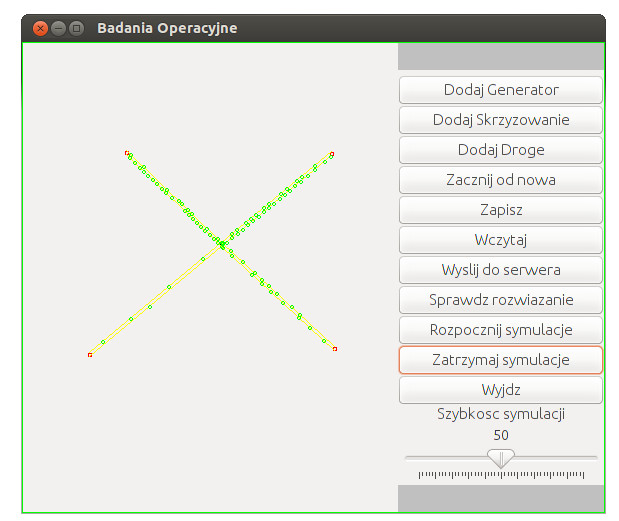
\includegraphics[width=90mm]{gui.jpg}
\caption{GUI dla części po stronie klienta}
\label{overflow}
\end{figure}

\subsection{Dodaj Generator}
    Gdy przycisk ten zostanie naciśnięty możemy za pomocą kliknięcia lewym przyciskiem myszy na obszarze do rysowania stworzyć generator. Zostanie on narysowany w klikniętym miejscu jako czerwone kółko.

\subsection{Dodaj Skrzyżowanie}
    Analogicznie jak w przypadku Generatora zostanie stworzony obiekt Skrzyżowanie. W klikniętym miejscu pojawi się czarne kółko.

\subsection{Dodaj Drogę}
    Po naciśnięciu przycisku "Dodaj Drogę" użytkownik może poprzez kliknięcie na dwóch skrzyżowaniach lub generatorze i skrzyżowaniu (najpierw jednym, a następnie na drugim), które zostało wcześniej narysowane, stworzyć nowy obiekt Droga. Gdy zostaną kliknięte dwa (wcześniej narysowane) obiekty typu Generator lub skrzyżowanie, pojawi się okno z zapytaniem o to ile samochodów może pomieścić droga, a następnie ile (w ciągu godziny) samochodów może przejechać przez tą drogę czyli intensywność zatłoczenia. Jeżeli jeden z zapytanych przez program parametrów nie zostanie podany lub będzie podany, ale w złym formacie np. użytkownik wpisze jakąś literę zamiast cyfry to obiekt nie zostanie stworzony. Po poprawnym podaniu wszystkich parametrów zostanie stworzony i narysowany obiekt typu droga. Narysowany jest podwójnie by było lepiej widać poruszające się samochody w obie strony. Jedna linia oznacza drogę w jedną stronę, a druga w drugą.

\subsection{Zacznij od nowa}
    Czyści całą narysowaną bądź wczytaną mapę.

\subsection{Zapisz}
    Zapisuje w wybranym przez użytkownika miaejscu na dysku narysowaną wcześniej mapę w postaci rysunku i list stworzonych obiektów.

\subsection{Wczytaj}
    Wczytuje z dysku wcześniej zapisaną mapę.

\subsection{Wyślij do serwera}
    Gdy narysujemy już bądź wczytamy mapę, musimy ją wysłać do włączonego wcześniej serwera żądanie, podając IP hosta, na którego komputerze jest włączony serwer, lub wpisując localhost jeśli mamy postawiony serwer lokalnie u siebie. Serwer zwraca nam ID jakie nadał temu żądaniu.

\subsection{Sprawdź rozwiązanie}
    Klikając ten przycisk, a następnie podając ID żądania, pytamy serwer czy dla danego żądania zostało wyliczone optymalne rozwiązanie. Serwer zwraca nam odpowiednią informację, która zostaje wyświetlona w okienku.

\subsection{Rozpocznij Symulację}
    Rozpoczęta zostanie symulacja poruszających się samochodów przedstawionych w postaci zielonych kółek. Symulacja jest przedstawiona wizualnie na narysowanej mapie. Współrzędne samochodów są pobierane co jakiś (bardzo krótki) czas przez co mamy wrażenie, że samochody poruszają się płynnie.

\subsection{Zatrzymaj Symulacje}
    Wstrzymuje wcześniej uruchomioną symulację. Wstrzymaną symulację możemy kontynuować po przez ponowne wciśnięcie przycisku "Rozpocznij Symulacje".

\subsection{Wyjdź}
    Przyciśnięcie tego przycisku powoduje wyjście z programu.

\subsection{Szybkość Symulacji}
    Jest to suwak umożliwiający nam wybór, jak szybko nasza symulacja ma się wykonywać. Dzięki temu możemy ją zwolnić aby lepiej zobaczyć rezultaty.

\section{Rezultaty}

W ramach projektu udało się utworzyć aplikacje, która jest w stanie znacząco poprawić przepływ pojazdów w symulowanych sieciach skrzyżowań. W ramach testów wydajnościowych uwotrzyliśmy szereg modeli. Dla każdego przypadku testowego wykonywaliśmy symulację przed i po zastosowaniu algorytmu kukułek. Przeprowadzenie symulacji wykazało, że obliczone poprzez zastosowanie algorytmu kukułek rozwiązania, były w stanie znacząco zredukować (często nawet o ponad 30-40\%) określoną przez nas funkcję celu. Wyniki, jak i mapki przedstawiające symulowane modele, zaprezentowane są poniżej.

\begin{figure}[ht!]
\centering
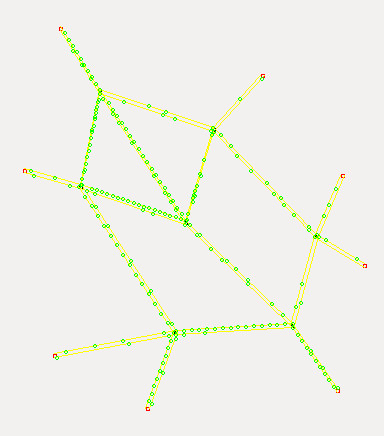
\includegraphics[width=90mm]{map1.jpg}
\caption{Wartość początkowa = 9143; Wartość końcowa = 5619}
\label{overflow}
\end{figure}


\begin{figure}[ht!]
\centering
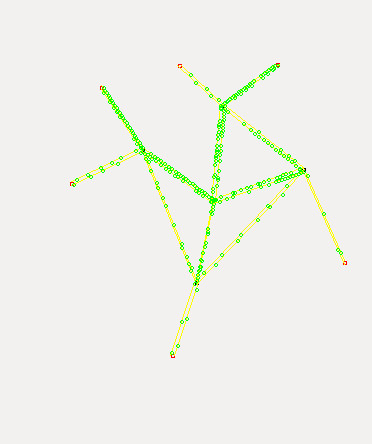
\includegraphics[width=90mm]{map2.jpg}
\caption{Wartość początkowa = 22231; Wartość końcowa = 15686 }
\label{overflow}
\end{figure}

\begin{figure}[ht!]
\centering
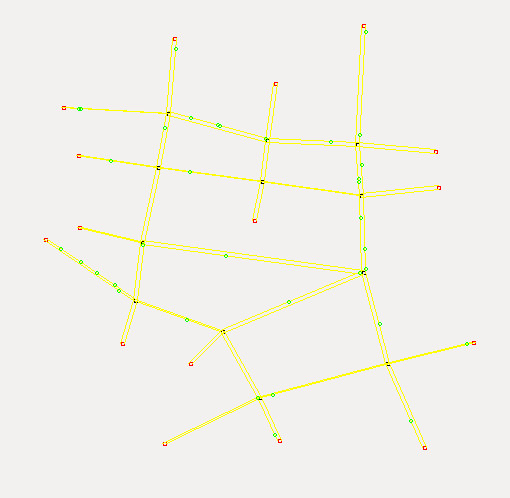
\includegraphics[width=90mm]{map3.jpg}
\caption{Wartość początkowa = 723; Wartość końcowa = 64}
\label{overflow}
\end{figure}

\begin{itemize}

\end{document} 